%!TEX program = xelatex
% Note: this template must be compiled with XeLaTeX rather than PDFLaTeX
% due to the custom fonts used. The line above should ensure this happens
% automatically, but if it doesn't, your LaTeX editor should have a simple toggle
% to switch to using XeLaTeX.

\documentclass[
  aspectratio=169, % Uncomment to use an aspect ratio of 16:9 (160 mm by 90 mm)
  %aspectratio=43, % Uncomment to use an aspect ratio of 4:3 (128mm by 96mm)
  t, % Top align all slide content by default
  onlytextwidth, % Typeset content in columns at text width
  10pt, % Default font size, use 10pt for the 16:9 aspect ratio and 8pt for the 4:3 aspect ratio
]{beamer}

\usepackage{../ImperialTheme/beamerthemeImperial} % Use the Imperial theme

\def\imagefolder{../ImperialTheme/Images/}

\title{Summary 1st term 2025} % Presentation title to appear on the title slide and left footers

\subtitle{} % Presentation subtitle to appear on the title slide

\author{Víctor Ballester} % Author name(s) to appear on the title slide

\date{\today} % Presentation date to appear on the title slide and right footers

\begin{document}

\begingroup
\setbeamercolor{background canvas}{bg=ICLBlue} % Slide background color
\setbeamercolor{title page title}{fg=white} % Title text color
\setbeamercolor{title page subtitle}{fg=white} % Subtitle text color
\setbeamercolor{author}{fg=white} % Author(s) text color
\setbeamercolor{date}{fg=white} % Date text color
\setbeamertemplate{title page}[logo]{\imagefolder/ICL_Logo_White.pdf} % Imperial logo color, use 'ICL_Logo_White.pdf' for white and 'ICL_Logo_Blue.pdf' for blue
\frame[plain, s]{\titlepage} % Output the title page with no footer ('plain') and vertically distributed text ('s')
\endgroup

\begin{frame}
  \frametitle{Domain}
  \begin{columns}[T] % [T] ensures correct vertical alignment
    \begin{column}{0.48\linewidth} % Left column
      \begin{itemize}
	\item $\delta^*$: measured at the upstream edge of the gap in a surface free of discontinuities.
	\item $Re_{\delta^*} = 1000$
	\item $L_i = 50\delta^*$
	\item $L_o = 500\delta^*$
	\item $h = 75\delta^*$
      \end{itemize}
    \end{column}
    \begin{column}{0.48\linewidth} % Right column
      \begin{itemize}
	\item $d = 4\delta^*$
	\item $w \in A\delta^*$, $A = \{10,\ldots,30\}$
	\item Inflow BC: Blasius profile
	\item Top BC: Far-field BC
	\item Wall BC: No-slip
	\item Outflow BC: Convective BC (Robin), or normal Neumann BC.
      \end{itemize}
    \end{column}
  \end{columns}
  {
  \centering
  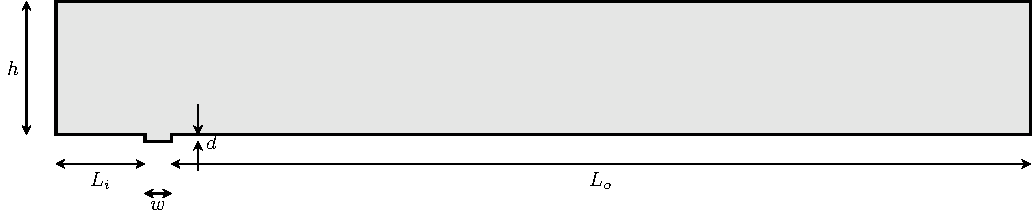
\includegraphics[width=1\textwidth]{../../Images/domain.pdf}
  }
\end{frame}
\begin{frame}
\frametitle{Current mesh}
{
  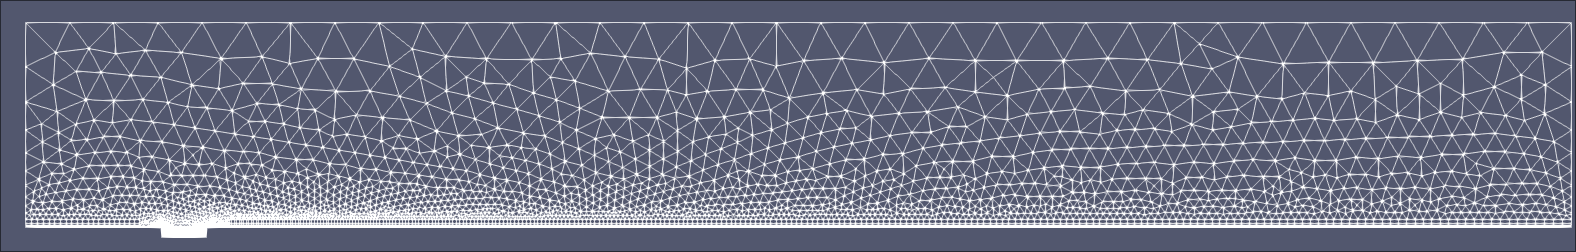
\includegraphics[width=0.95\textwidth]{Images/mesh_full.png}
  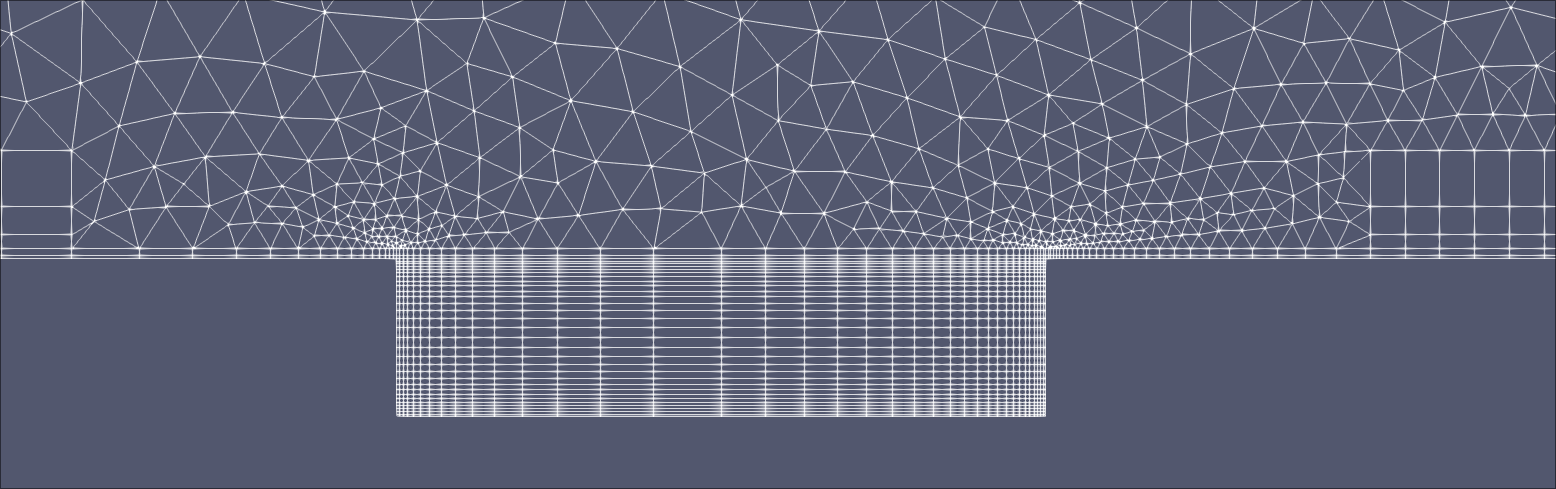
\includegraphics[width=0.95\textwidth]{Images/mesh_gap.png}
}

\end{frame}
\begin{frame}
  \frametitle{Study - range of $w$}
  \begin{itemize}
    \item For $w \leq 16.4\delta^*$, we observe a steady state from nonlinear simulations (``global" attractor).
    \item As we increase $w\geq 16.5\delta^*$, we observe a divergent behavior. Thus, to do LSA with those cases we have to make use of Selective Frequency Damping (SFD) (e.g. control theory) to get a locally stable baseflow.
    \item \textbf{Conjecture}: the critical width at $d=4\delta^*$ lies in the interval $(16.4\delta^*, 16.5\delta^*)$ (up to numerical sensitivity).
  \end{itemize}
\end{frame}
\begin{frame}
  \frametitle{Unstable baseflows}
  {
    \begin{center}
      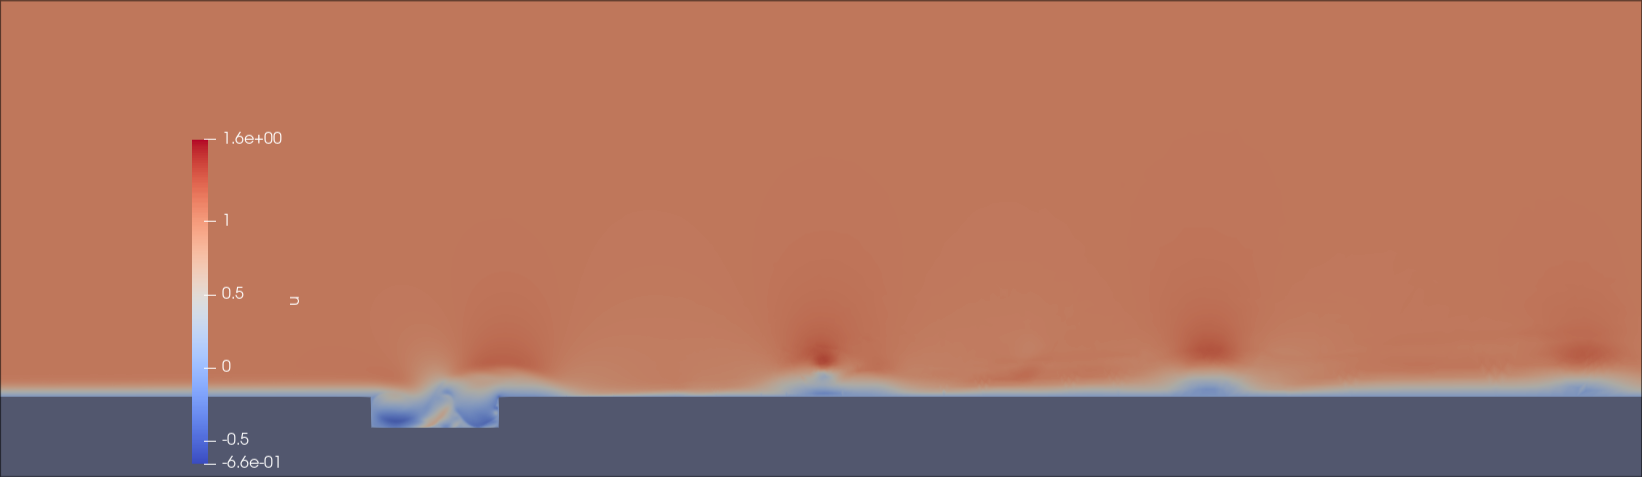
\includegraphics[width=0.6\linewidth]{Images/dns16.5.png}

      u-component of dns simulations with $w = 16.5\delta^*$ at time $t \sim 11\,500$.

      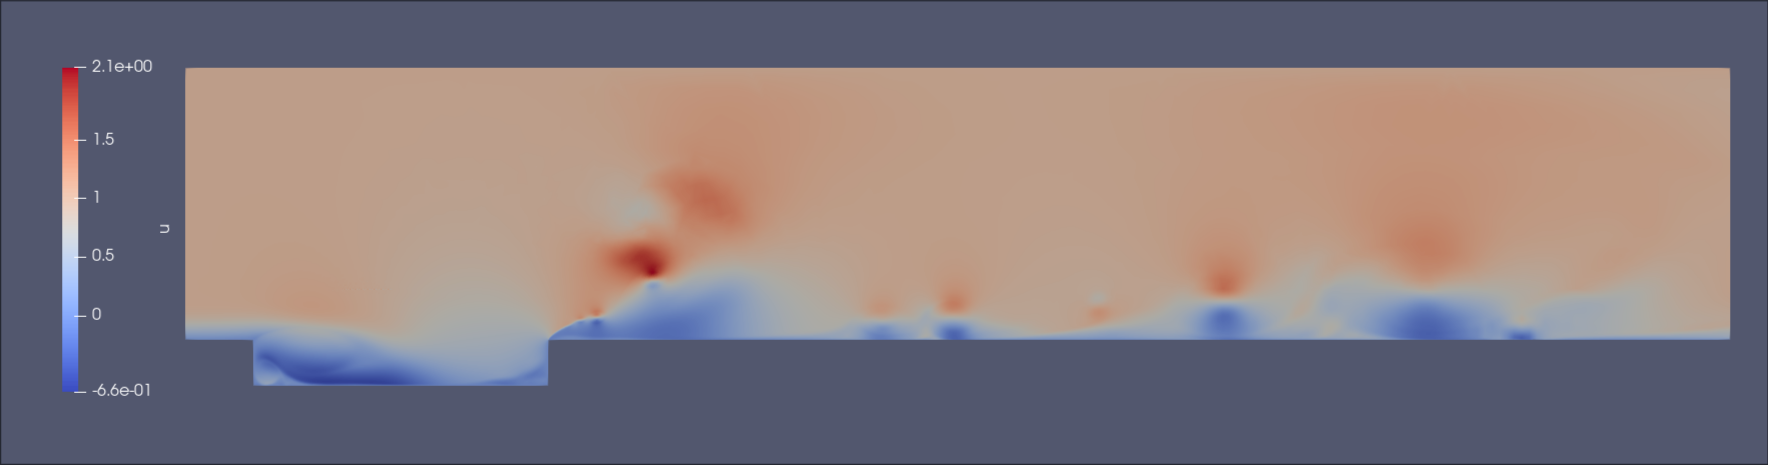
\includegraphics[width=0.6\linewidth]{Images/dns26.png}

      u-component of dns simulations with $w = 26\delta^*$ at time $t \sim 1500$ (old run with a short domain).
    \end{center}

  } 
\end{frame}
\begin{frame}
  \frametitle{Stable baseflows}
  \begin{columns}[T] % [T] ensures correct vertical alignment
    \begin{column}{0.48\linewidth} % Left column
      {
	\centering
	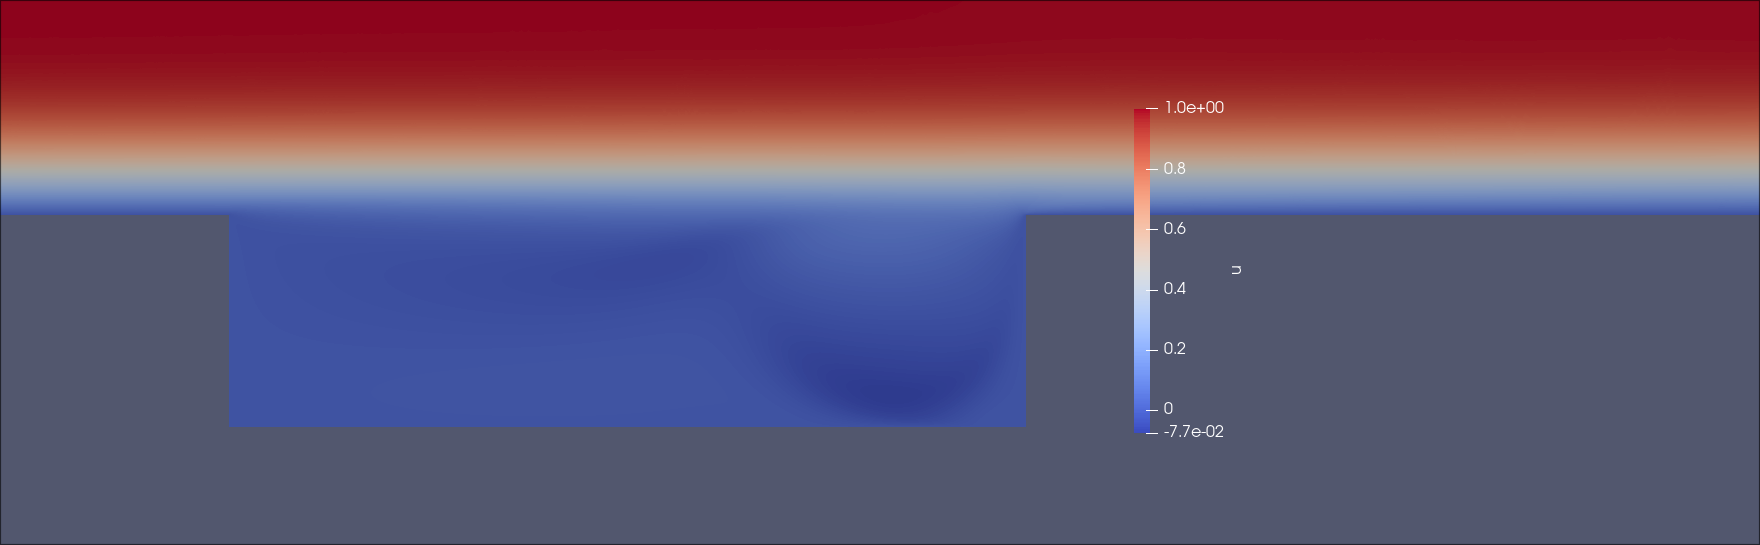
\includegraphics[width=\linewidth]{Images/ubf15.png}
	u-component \emph{natural} baseflow with $w = 15\delta^*$

	\centering
	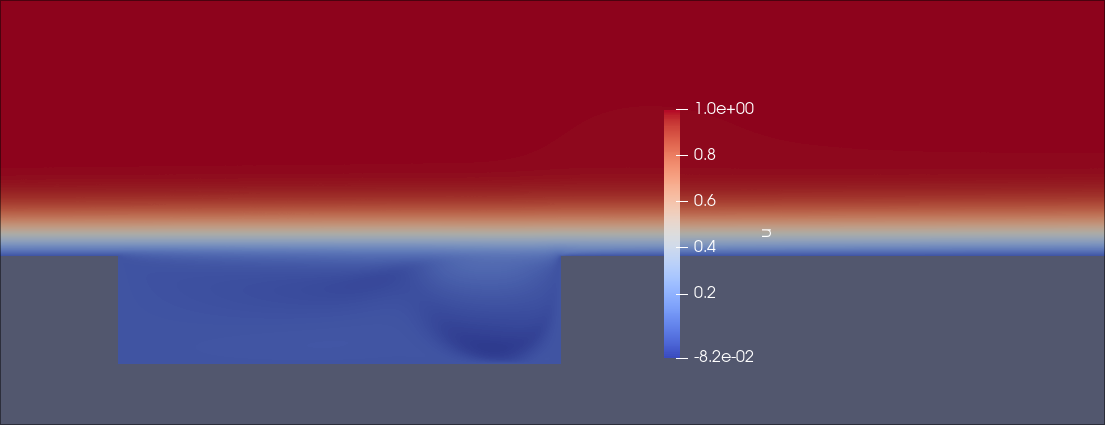
\includegraphics[width=\linewidth]{Images/ubf16.5.png}
	u-component SFD baseflow with $w = 16.5\delta^*$
      }
    \end{column}
    \begin{column}{0.48\linewidth} % Right column
      {
	\centering
	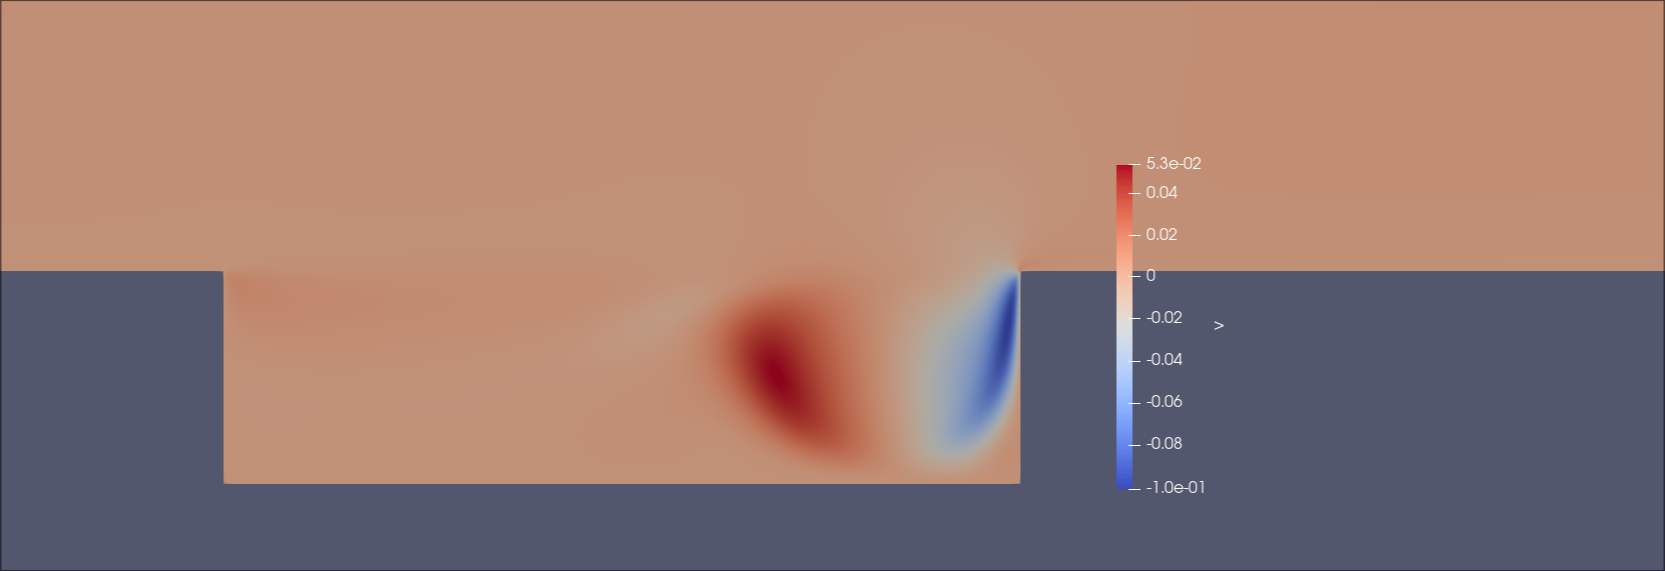
\includegraphics[width=\linewidth]{Images/vbf15.png}
	v-component \textit{natural} baseflow with $w = 15\delta^*$

	\centering
	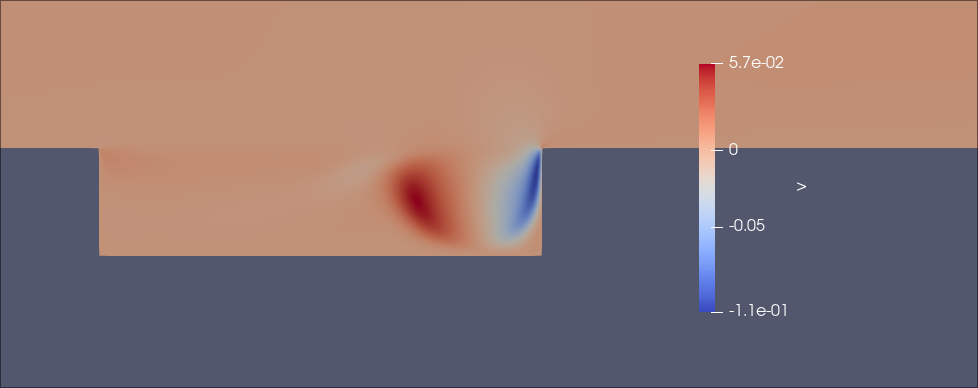
\includegraphics[width=\linewidth]{Images/vbf16.5.png}
	v-component SFD baseflow with $w = 16.5\delta^*$
      }
    \end{column}
  \end{columns}
\end{frame}
\begin{frame}
  \begin{columns}[T] % [T] ensures correct vertical alignment
    \begin{column}{0.48\linewidth} % Left column
      {
	\centering
	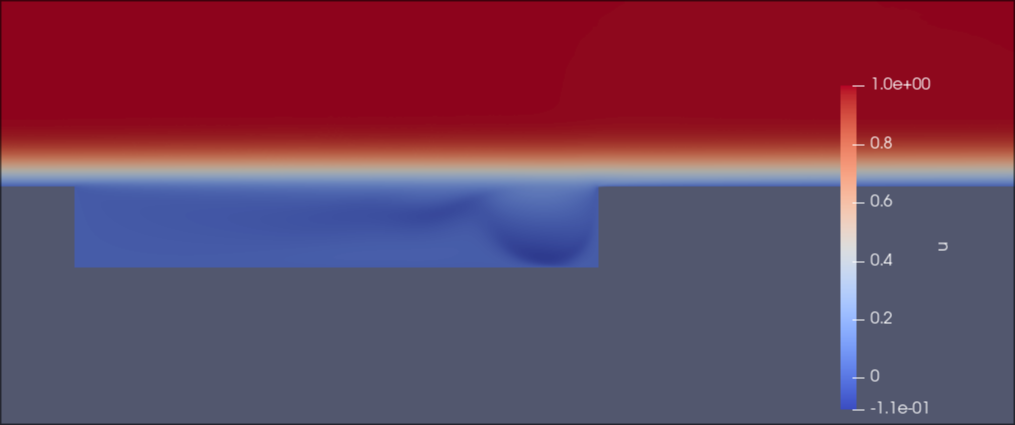
\includegraphics[width=\linewidth]{Images/ubf26.png}
	u-component SFD baseflow with $w = 26\delta^*$
      }
    \end{column}
    \begin{column}{0.48\linewidth} % Right column
      {
	\centering
	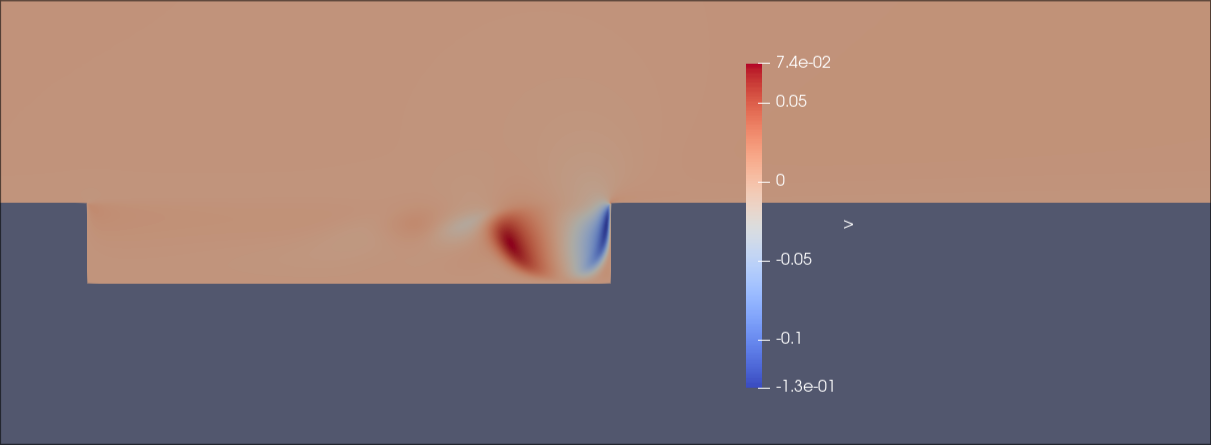
\includegraphics[width=\linewidth]{Images/vbf26.png}
	v-component SFD baseflow with $w = 26\delta^*$
      }
    \end{column}
  \end{columns}
      {
	\centering
	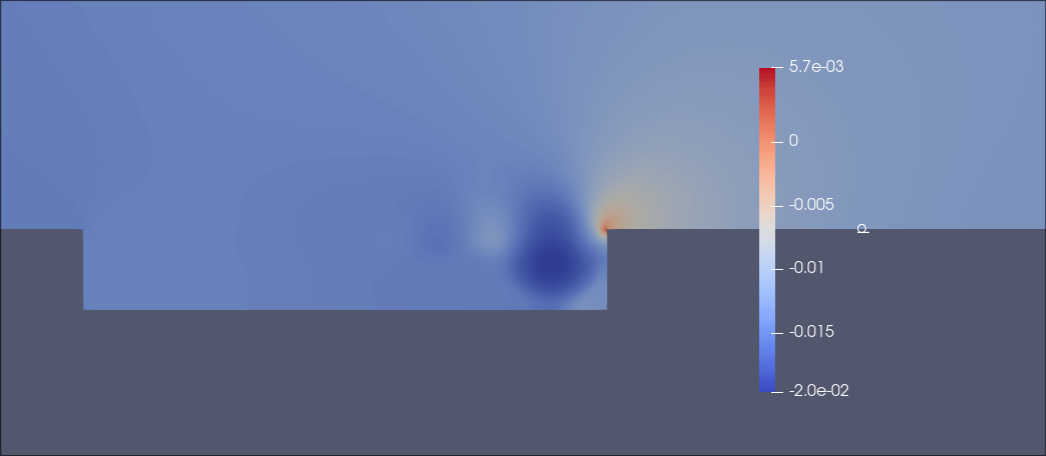
\includegraphics[width=0.48\linewidth]{Images/pbf26.png}

	\centerline{
	pressure SFD baseflow with $w = 26\delta^*$}
      }
\end{frame}
\begin{frame}
  \frametitle{Linear stability analysis}
  \begin{columns}[T] % [T] ensures correct vertical alignment
    \begin{column}{0.48\linewidth} % Right column
      \textbf{Case $w = 15\delta^*$}. Most unstable mode:
      \begin{itemize}
	\item Growth rate: $-0.00279$
	\item Frequency: $\pm0.00304$
      \end{itemize}
      Comments:
      \begin{itemize}
	\item This is not a TS mode. We observe a huge mode in the BL.
	\item The magintude of the fields is much higher inside the gap than on the BL (around 2-10 orders, depending on the $x$-position in the BL)

      \end{itemize}
    \end{column}
    \begin{column}{0.48\linewidth} % Left column
      {
	\centering
	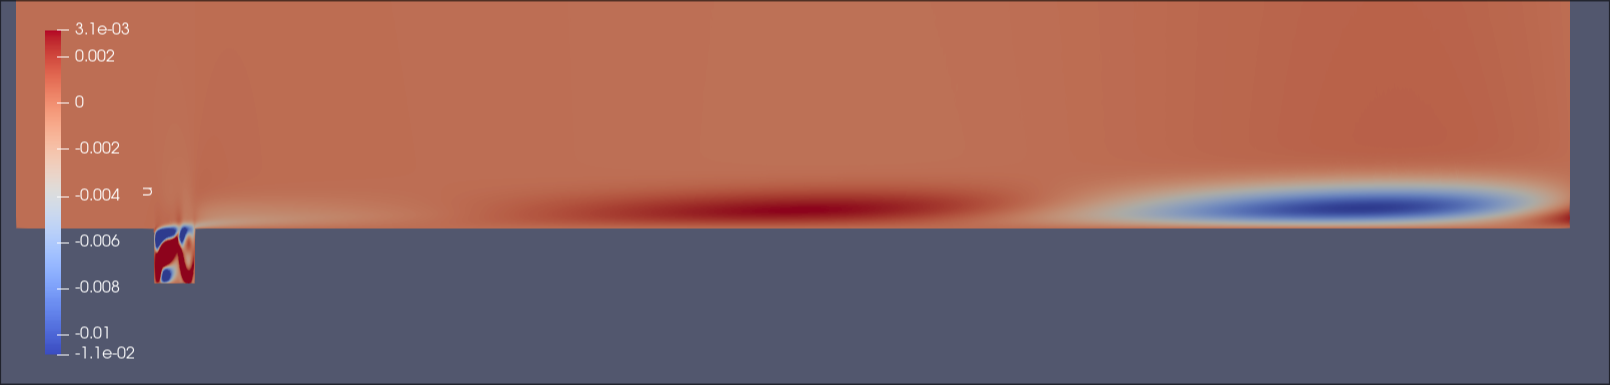
\includegraphics[width=\linewidth]{Images/uem15.png}
	u-component of the most unstable eigenmode with $w = 15\delta^*$ (domain scaled in the $x$-dir by 0.1)

      }
      {
	\centering
	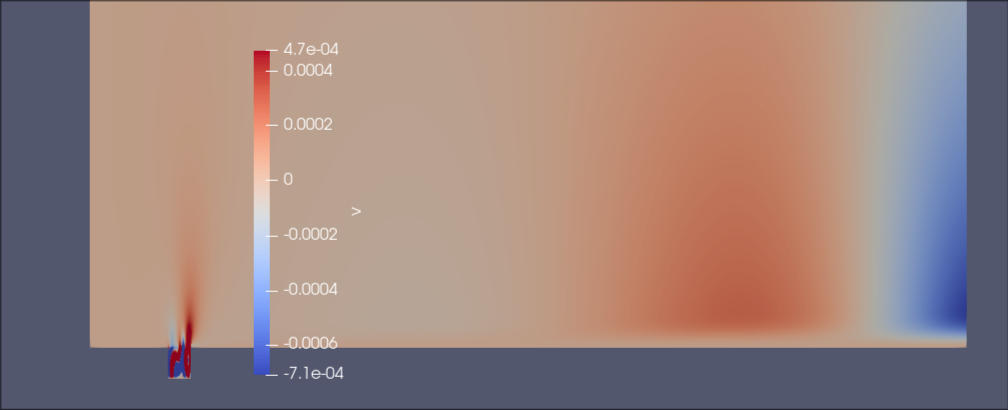
\includegraphics[width=\linewidth]{Images/vem15.png}
	v-component of the most unstable eigenmode with $w = 15\delta^*$ (domain scaled in the $x$-dir by 0.1)

      }
    \end{column}
  \end{columns}
\end{frame}
\begin{frame}
  \frametitle{Linear stability analysis}
  \begin{columns}[T] % [T] ensures correct vertical alignment
    \begin{column}{0.48\linewidth} % Right column
    \textbf{Case $w = 16.5\delta^*$} (very similar to $w=15\delta^*)$. Most unstable mode:
      \begin{itemize}
	\item Growth rate: $-0.00258$
	\item Frequency: $\pm0.00276$
      \end{itemize}
      Comments:
      \begin{itemize}
	\item We do \textbf{not} observe a mode with positive growth rate, which suggests (up to numerical sensitivity and other possible errors) that the nature of the instability would be nonlinear instead of linear.
      \end{itemize}
     \end{column}
    \begin{column}{0.48\linewidth} % Left column
      {
	\centering
	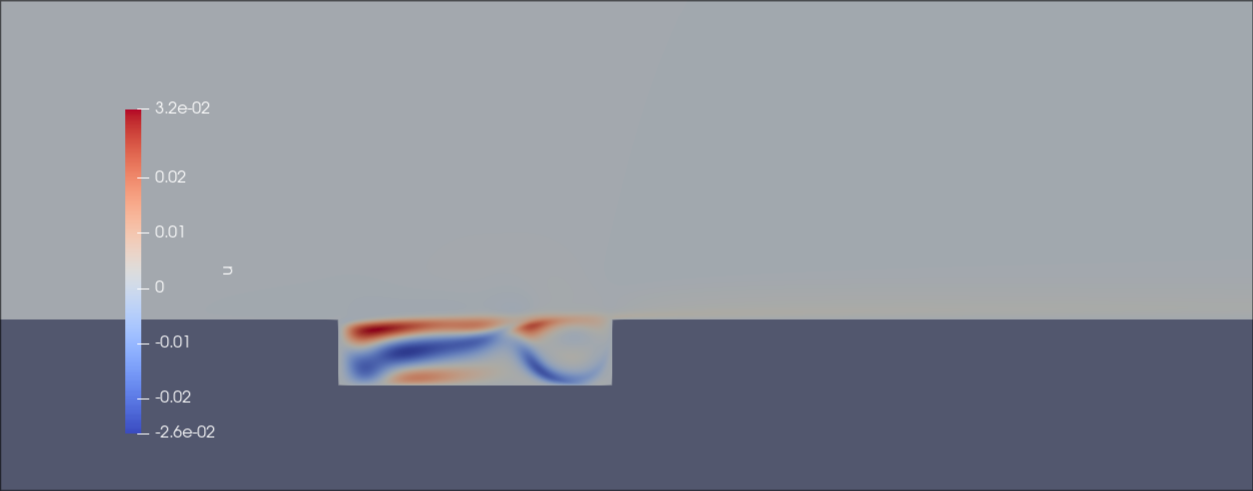
\includegraphics[width=0.9\linewidth]{Images/uem16.5.png}
	u-component of the most unstable eigenmode with $w = 16.5\delta^*$ (emphasizing colors in the gap)
      }
      {
	\centering
	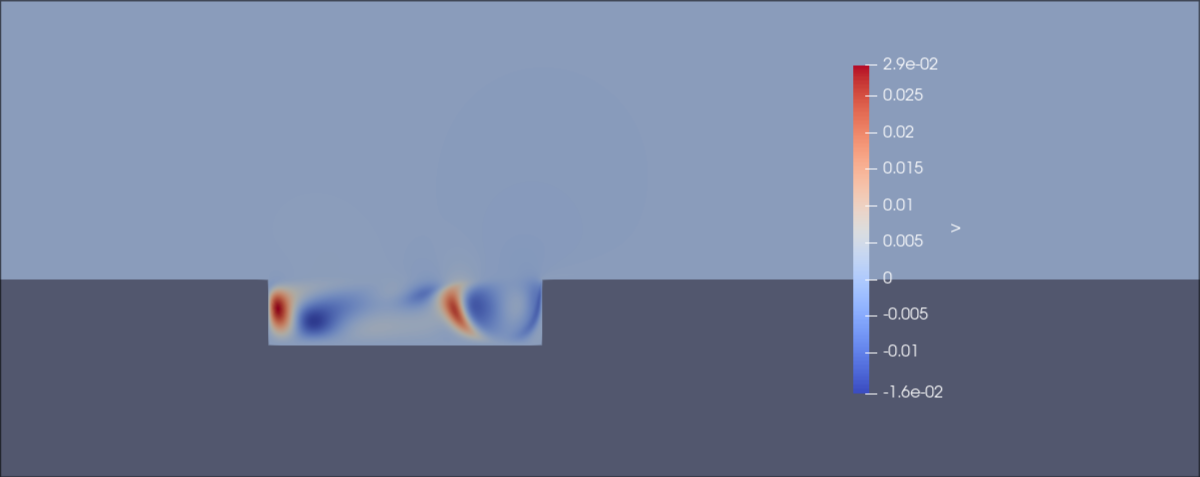
\includegraphics[width=0.9\linewidth]{Images/vem16.5.png}
	v-component of the most unstable eigenmode with $w = 16.5\delta^*$ (emphasizing colors in the gap)
      }
    \end{column}
  \end{columns}
\end{frame}
\begin{frame}
  \frametitle{Linear stability analysis}
  \begin{columns}[T] % [T] ensures correct vertical alignment
    \begin{column}{0.48\linewidth} % Right column
    \textbf{Case $w = 26\delta^*$}. Most unstable mode:
      \begin{itemize}
	\item Growth rate: $0.00859$
	\item Frequency: $\pm0.00887$
      \end{itemize}
      Comments:
      \begin{itemize}
	\item This mode looks like the result of an absolute instability in the gap because the amplitude of the waves decreases as they move downstream.
      \end{itemize}
     \end{column}
    \begin{column}{0.48\linewidth} % Left column
      {
	\centering
	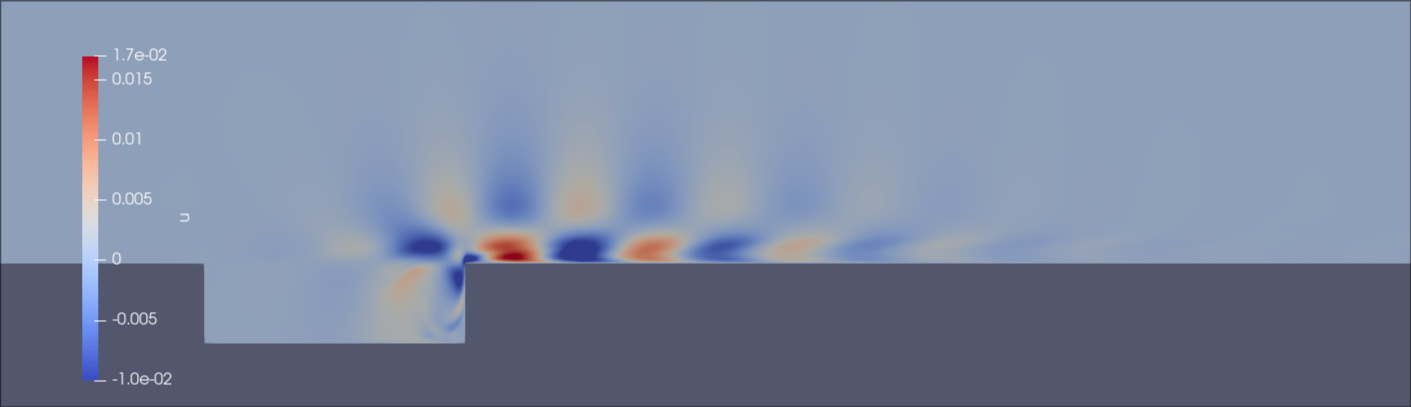
\includegraphics[width=0.85\linewidth]{Images/uem26.png}
	u-component of the most unstable eigenmode with $w = 26\delta^*$ (domain scaled in the $x$-dir by 0.5)

      }
      {
	\centering
	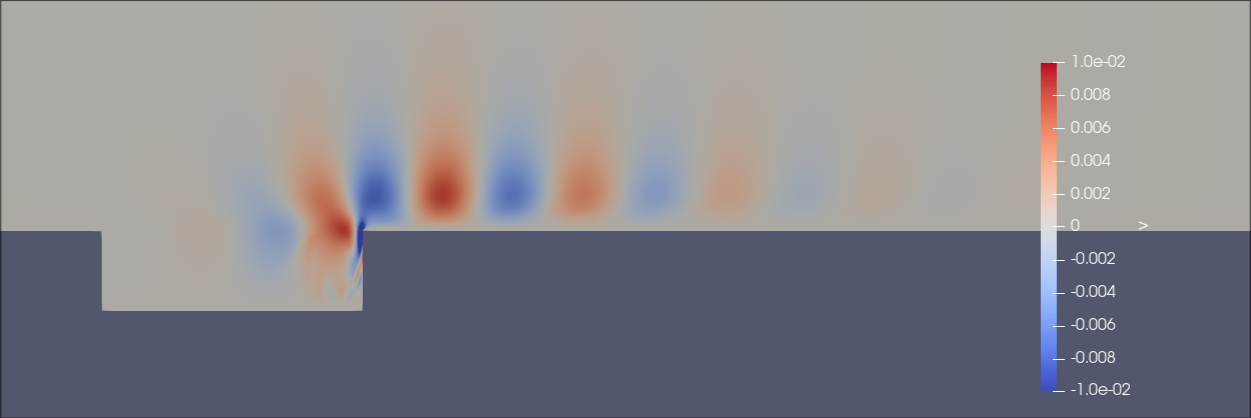
\includegraphics[width=0.85\linewidth]{Images/vem26.png}
	v-component of the most unstable eigenmode with $w = 26\delta^*$ (domain scaled in the $x$-dir by 0.5)

      }
    \end{column}
  \end{columns}
\end{frame}
\begin{frame}
  \frametitle{Nature of the instability (work in progress)}
  \begin{itemize}
  \item Runs doing global stability analysis from a baseflow just above the critical width where non-steadiness shows up on dns (e.g $w_{critical}|_{d= 4\delta^*}\in (16.4\delta^*,16.5\delta^*)$ show eigenmodes with a \textbf{negative} growth rate.
  \item We did check that adding those modes to the baseflow as initial conditions in the nonlinear solver leads to a steady solution (we ran that for $w=16.5\delta^*$ and $w=18\delta^*$). This does \textbf{not} happen though for $w=26\delta^*$.
  \end{itemize}
\end{frame}
\begin{frame}
  \frametitle{Coherence between DNS and LSA}
  Let 
  $$
  \boldsymbol{\varphi}(t;(u_0, v_0))=(\varphi_u(t;(u_0,v_0)),\varphi_v(t;(u_0,v_0)))
  $$ the flow of NS eqs at time $t$ with initial conditions $(u_0,v_0)$. Let $(U,V)$ be the baseflow of our system and $(\tilde{u},\tilde{v})$ the most unstable eigenmode with $\lambda$ the respective growth rate. We plot the following quantities
  \begin{align*}
  t\mapsto \frac{\|{\varphi_u(t;(U+\tilde{u},V+\tilde{v}))-U\|}_{L^2}}{\|{U}\|_{L^2}}\\
  t\mapsto \frac{\|{\varphi_v(t;(U+\tilde{u},V+\tilde{v}))-V\|}_{L^2}}{\|{V}\|_{L^2}}
  \end{align*}
  for different $w$. This should tell us how the energy of the perturbation evolves in time. We compare this with the theoretical evolution of the energy based on LSA, which goes as $\|u_0\|_{L^2}e^{\lambda t}$ and $\|v_0\|_{L^2}e^{\lambda t}$, respectively.
\end{frame}
\begin{frame}
  \textbf{Case $w=26\delta^*$}

  \begin{columns}[T] % [T] ensures correct vertical alignment
    \begin{column}{0.48\linewidth} % Right column
      {
	\centering
	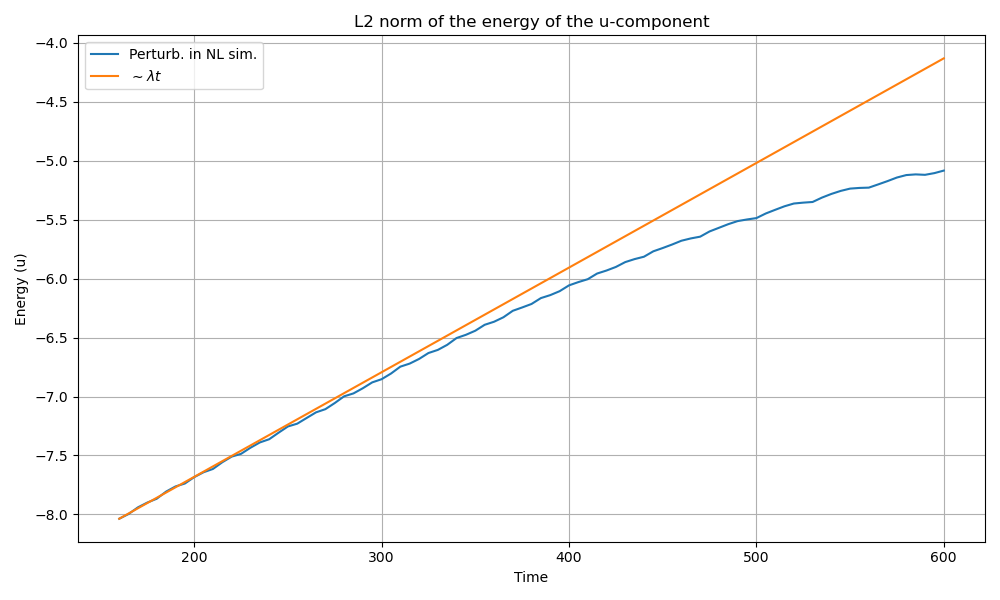
\includegraphics[width=\linewidth]{Images/energyL2_error_u26.png}
	$u$-component
      }
    \end{column}
    \begin{column}{0.48\linewidth} % Left column
      {
	\centering
	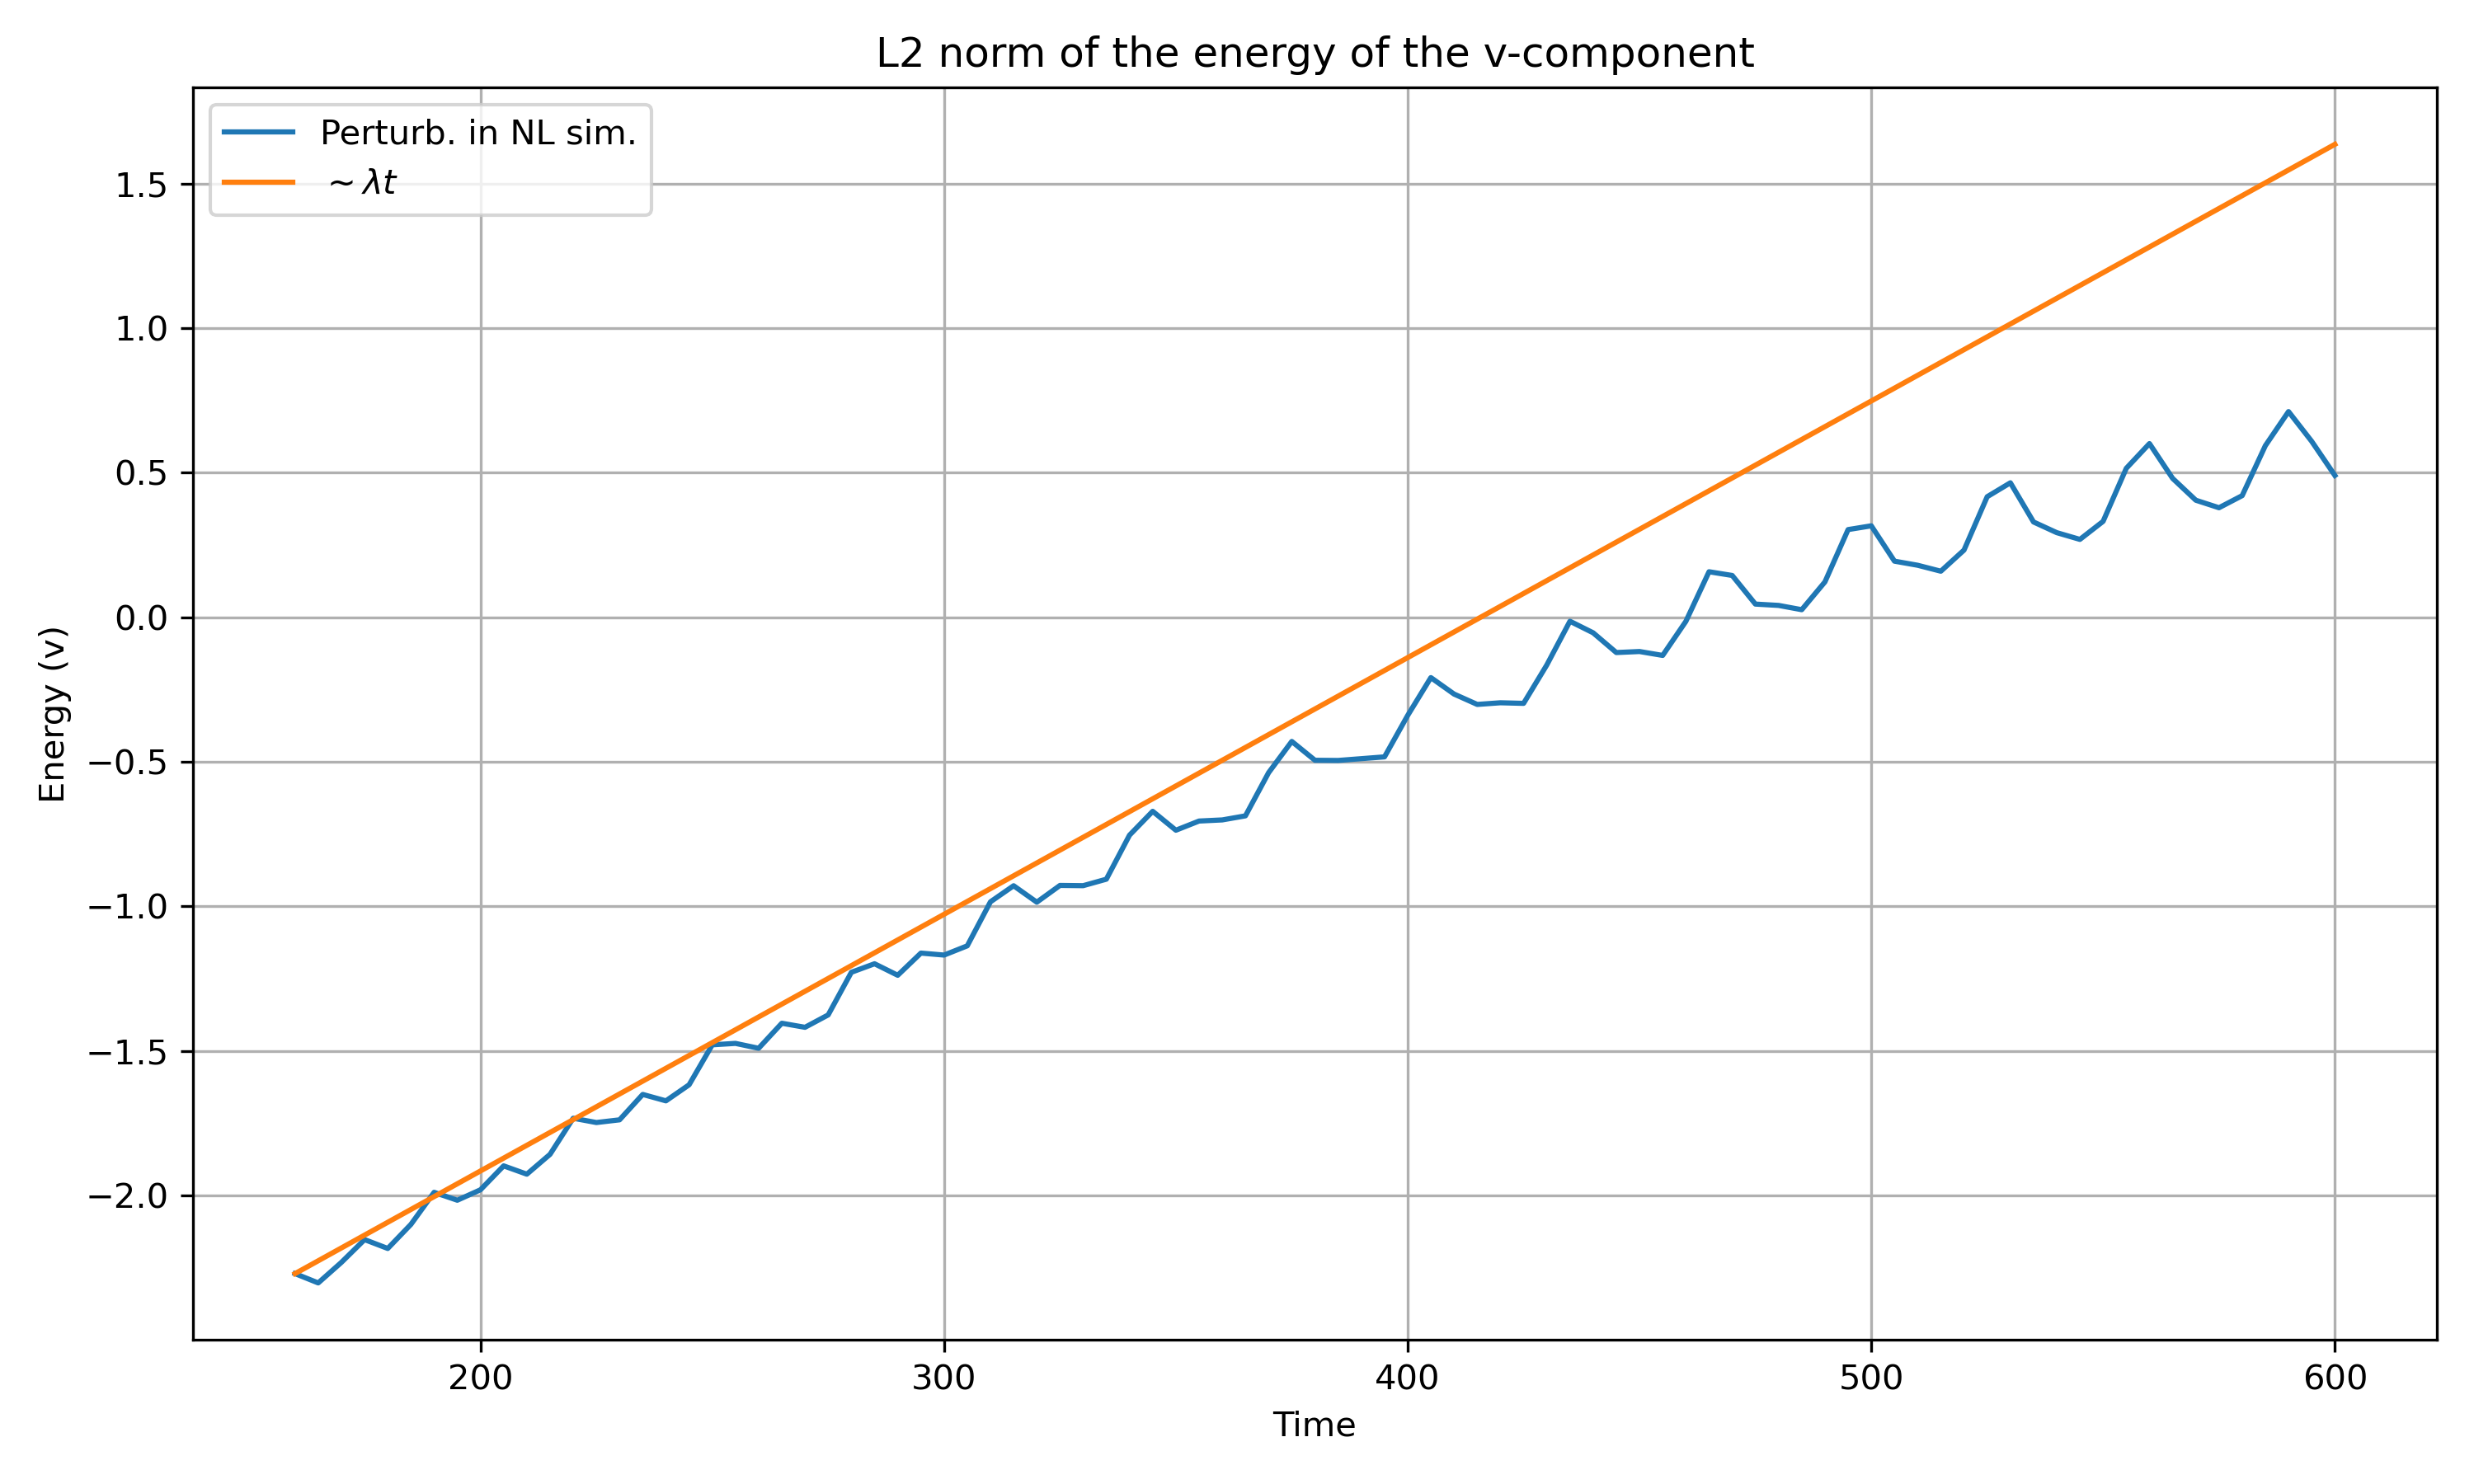
\includegraphics[width=\linewidth]{Images/energyL2_error_v26.png}
	$v$-component
      }
    \end{column}
  \end{columns}
  \begin{itemize}
    \item We are plotting the log of the energy.
    \item Initially the nonlinear results fits well the linear prediction after which ($t \sim 450$) the nonlinear effects start to contribute significantly.
  \end{itemize}
\end{frame}
\begin{frame}
  \textbf{Case $w=15\delta^*$} (similar to $w=16.5\delta^*$)

  \begin{columns}[T] % [T] ensures correct vertical alignment
    \begin{column}{0.48\linewidth} % Right column
      {
	\centering
	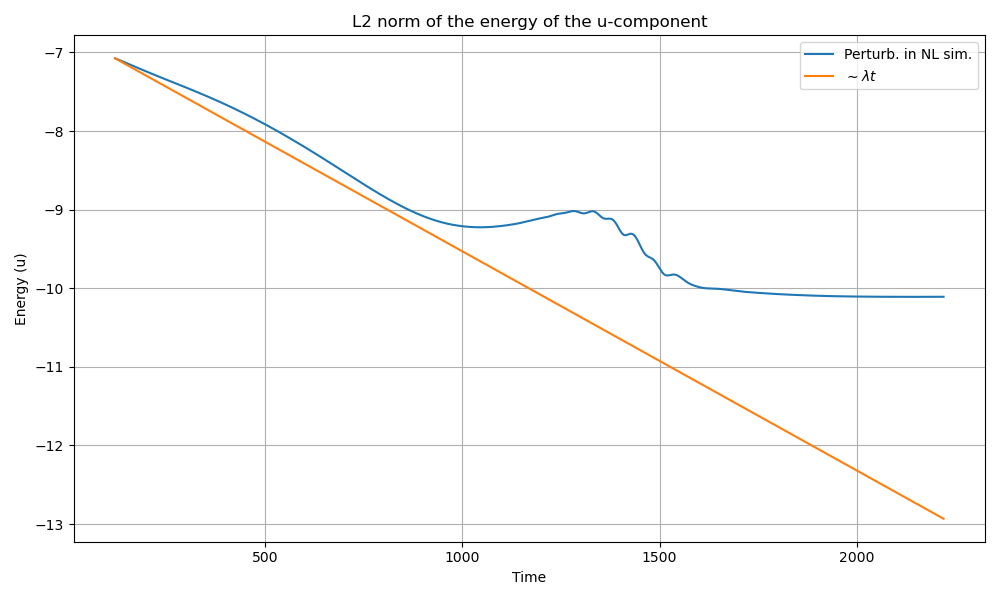
\includegraphics[width=\linewidth]{Images/energyL2_error_u15.png}
	$u$-component
      }
    \end{column}
    \begin{column}{0.48\linewidth} % Left column
      {
	\centering
	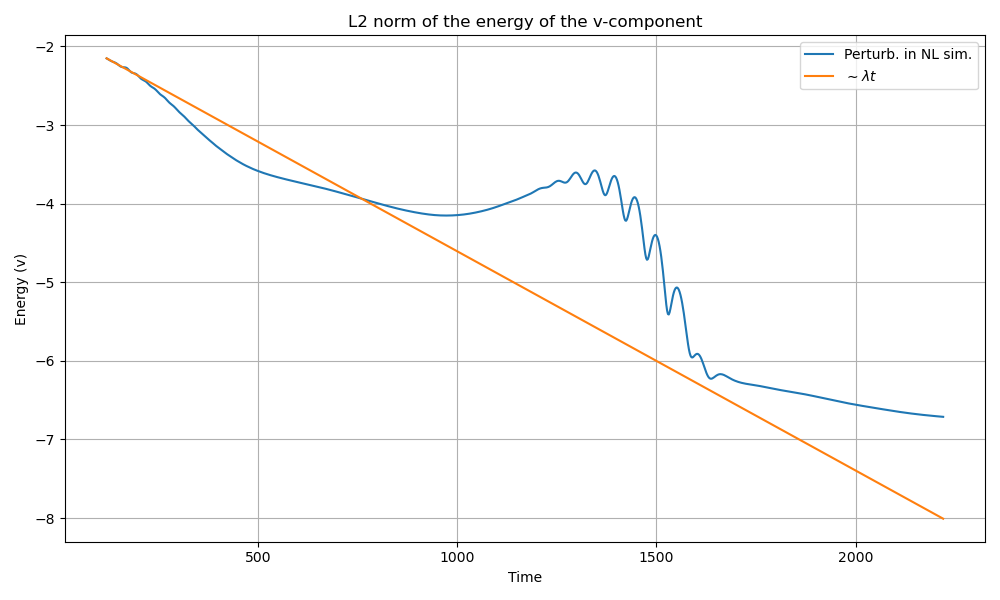
\includegraphics[width=\linewidth]{Images/energyL2_error_v15.png}
	$v$-component
      }
    \end{column}
  \end{columns}
  \begin{itemize}
    \item We are plotting the log of the energy.
    \item The fit is less nicer, and we observe a weird bump appearing on the middle of the time interval considered.
  \end{itemize}
\end{frame}
\begin{frame}
  \frametitle{The bump}
  $u$-component the perturbed system at different times (domain scaled in the $x$-dir)
   \begin{columns}[T] % [T] ensures correct vertical alignment
    \begin{column}{0.48\linewidth} % Right column
      {
	\centering
	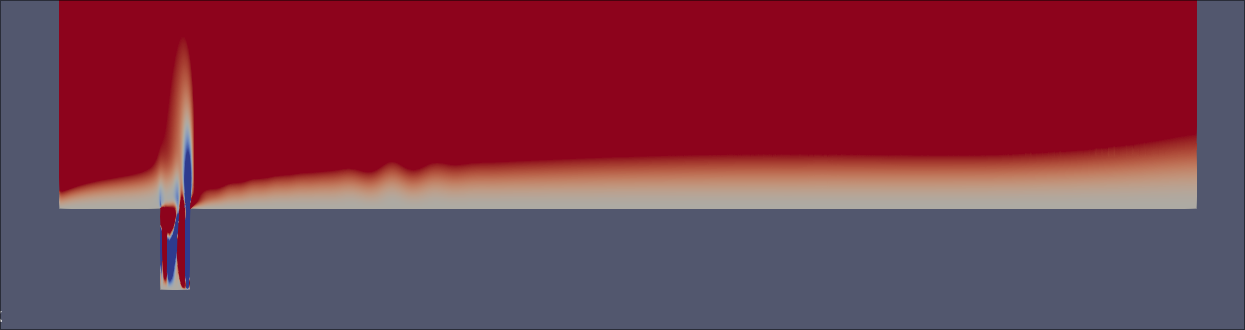
\includegraphics[width=\linewidth]{Images/1.png}
      }
      {
	\centering
	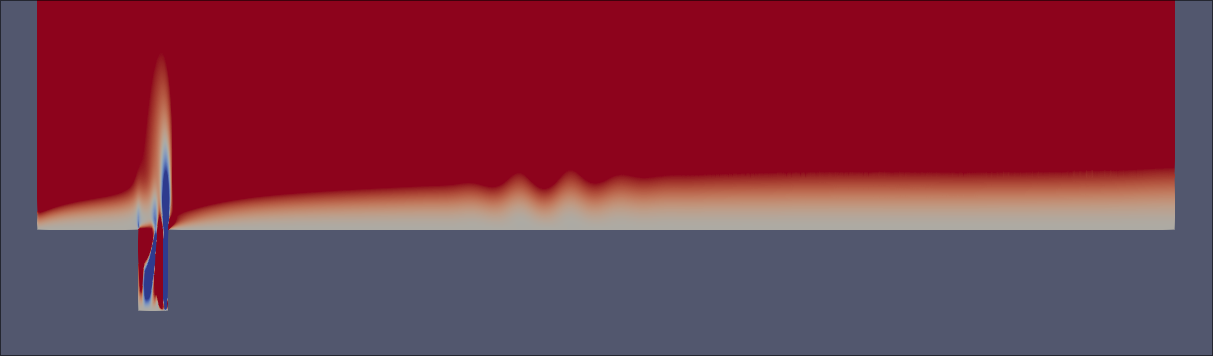
\includegraphics[width=\linewidth]{Images/2.png}
      }
      {
	\centering
	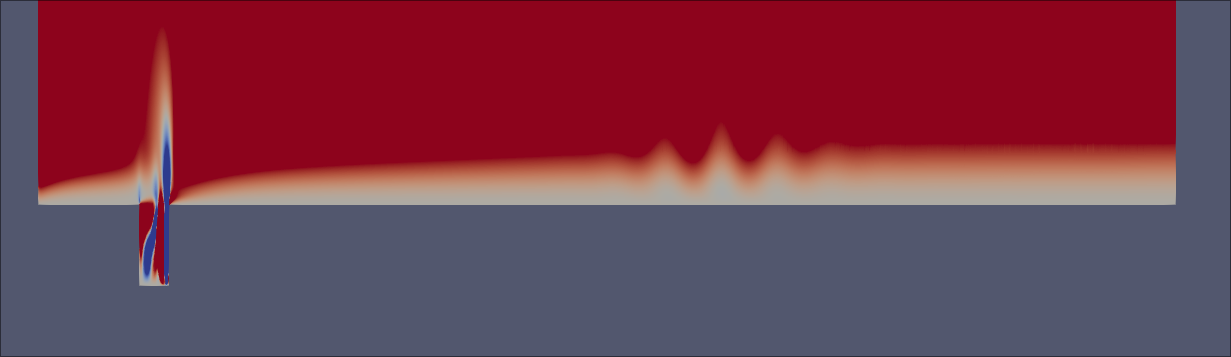
\includegraphics[width=\linewidth]{Images/3.png}
      }
    \end{column}
    \begin{column}{0.48\linewidth} % Left column
       {
	\centering
	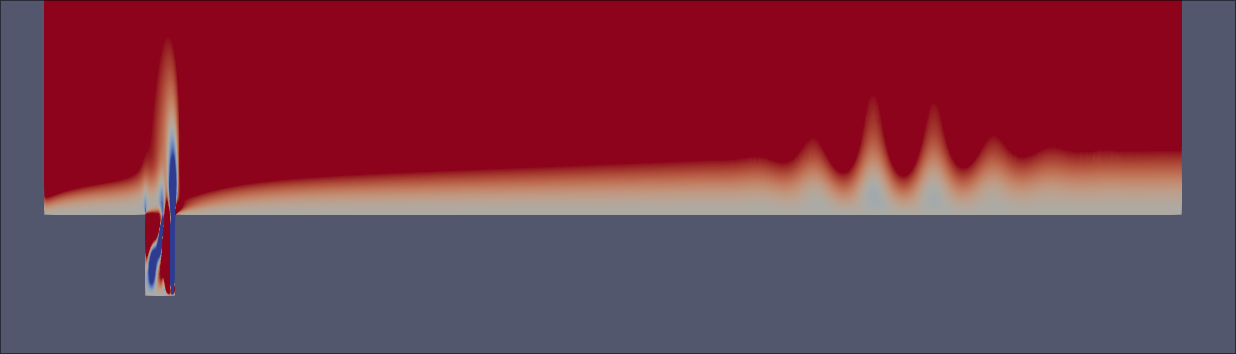
\includegraphics[width=\linewidth]{Images/4.png}
      }
      {
	\centering
	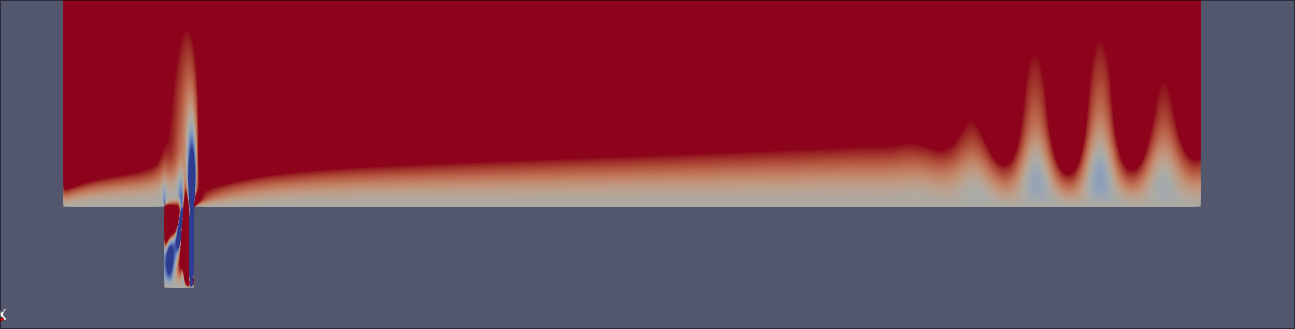
\includegraphics[width=\linewidth]{Images/5.png}
      }
      {
	\centering
	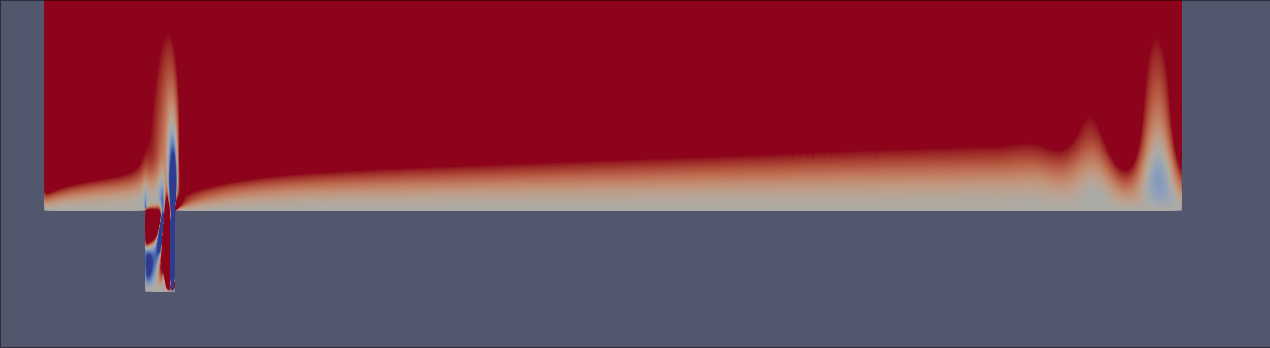
\includegraphics[width=\linewidth]{Images/6.png}
      }
    \end{column}
  \end{columns}
\end{frame}
\begin{frame}
  \frametitle{The bump}
  \begin{itemize}
    \item Looks like the modes may be providing the system with enough energy inside the gap to trigger the convective instability nature of the system. \textbf{Why?} The stable modes computed for $w=15\delta^*$ and $w=16.5\delta^*$ showed bigger magnitudes inside the gap than on the BL.
  \end{itemize}
\end{frame}
\begin{frame}
  \frametitle{Questions}
  \begin{itemize}
    \item What range of $d$ should we consider in the future?
    \item Should we first move to 3D case or to 2D compressible case?
  \end{itemize}
\end{frame}

\end{document}
